\documentclass[11pt,a4paper,onesides]{report}
\usepackage{graphicx}
\usepackage[parfill]{parskip}
\DeclareGraphicsExtensions{.pdf,.png,.jpg}



\begin{document}

\title{User Interface and Embedded System  \\ Technical Report}
\author{Paul Glotfelter}
\date{August 2014}

\maketitle

\tableofcontents

\addcontentsline{toc}{section}{Introduction}

\renewcommand{\chaptername}{Section}

\section*{Introduction}

This report covers the research, design, analysis, and prototyping of the team 2 Automated Bike Rental Station (ABRS).  In particular, the report discusses the initial requirements and expectations, the research to investigate the initial criteria, the analysis of the proposed model, and the prototyping of the proposal involving the embedded system and user interface of the project.  

\chapter{Initial Requirements}

The initial requirements were set forth in the form of a system from which customers can rent bicycles.  The purpose of this product is to enrich the communication and relationship between York College and its surrounding community.  To facilitate this project, certain major specifications are required from the ABRS system.  The bike rack must be able to operate year-round, customers return bikes to the same stations from which they were rented, and the ABRS must be able to sufficiently power itself when a grid connection is unavailable.  These criteria present unique problems to each engineering group working on the project.  However, this report specifically covers the requirements the criteria imposed on the computer engineering portion of the ABRS.  

\section{General Guidelines}

The general guidelines are: the ABRS must consist of a kiosk (a central unit housing the display and handling customer interactions) and one to five bike modules.  Each bike module will house five bikes with individual locking stations for each one.  The entire unit must be generally resilient to physical damage.  In addition, it must be completely safe for operation with young children as well as adults.    

\section{Operating Conditions}

In order for the bike system to operate year round, the components selected for the rack must be able to withstand the extreme temperature variations of the hot and cold weather experienced in the York, Pennsylvania area.  The ABRS must also be intuitive and simple to use in each of these weather conditions.  Additionally, the ABRS may be located in city areas.  So, its components should be highly resistant to vandalism and theft. 

\section{Return Procedure}

As this is a product being designed for the general consumer, the end result is to be as intuitive and simple as possible.  Thus, when customers return bicycles, the checkout procedure must be straightforward.  Under optimal conditions, the customers will simply return the bicycle to the ABRS and their account will be appropriately charged.  In order for the system to discern which bike is being returned, it must be able to uniquely identify bikes.

\section{System Power}

 The ABRS system aims to be totally self-sufficient in terms of supplying power to the components.  However, it must also be able to connect to the grid when necessary.  Therefore, the components must be selected with these goals in mind.  That is, the power consumption of the components must be low so that the system can be self-sufficient.  In addition, power-saving protocols for the UI may also be required.  

\chapter{Initial Developments}

After receiving the requirements and laying out some criteria, developments were made for the communication protocol, user interactions with the kiosk, and locking mechanisms.

\section{Communications Protocol}

In general, the system can be described as a central kiosk unit communicating by some protocol to each of the individual bike modules.  This description is the core of the ABRS from an engineering perspective.  To facilitate easy of programming and quick prototyping, a wired approach was selected.  That is, a scheme in which the kiosk is directly connected to each of the bike modules and directly controls the bike locking mechanisms.  

The initial thought was to use wireless communication for this purpose.  Wireless communication ubiquitous in modern systems.  In addition, it allows for easy communication between the kiosk and each bike module.  However, it does present an entirely new set of problems to address: the wireless communications must be encrypted and each bike module must be equipped with an embedded component capable of handling wireless transmission, adding additional cost to the system.  The largest issue with wireless is the time required to develop software to ensure the security of the system, and the conclusion is that security protocols and, thus, wireless transmission are outside the scope of this capstone iteration.  

Because of the issues with wireless communication,  it is far more efficient in terms of time and cost to use a wired approach.  In particular, a scheme in which the kiosk is directly connected to each of the bike modules and directly controls the bike locking mechanisms (discussed further in section ???), resulting in the rough system model shown in Figure 2.1. 

%0.6 seems to be a really good size for figures :)

\begin{figure}[h]
	\begin{center}
		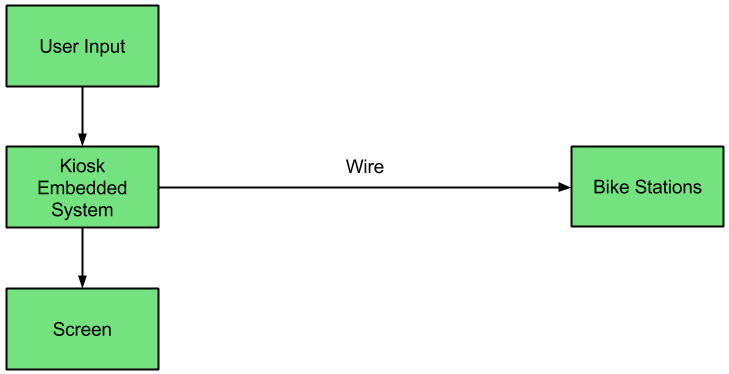
\includegraphics[scale = 0.6]{initial-diagram}
	\end{center}
\caption{A preliminary diagram of the system}

\end{figure}

The communication protocol's purpose is twofold: allowing the kiosk to unlock bikes and allowing the stations to supply the kiosk with bike information.  Generally, there are two major use cases in which the protocol is used: a user rents a bike and a user returns a bike.  The case for a user renting a bike is as follows: 

\begin{enumerate}

  \item User attempts to rent a bike
  \item Kiosk polls each station to determine which bikes are available
  \item Kiosk selects the first available bike and sends an unlock command its respective station
  \item Locking mechanism controller releases the bike
  \item Kiosk informs user that a bike has been dispensed and directs them to the station

\end{enumerate}

\section{User Interactions}

The chosen display for the ABRS is an industrial LCD screen.  The manner in which the system interacts with the user is the single most important goal for the ABRS to achieve.  The system must offer an interface that is aesthetically pleasing and intuitive to navigate.  These criteria guided the team to initially discuss using a touchscreen for the kiosk display.  However, background research revealed that the temperature ranges in York, Pennsylvania would be too harsh for a touchscreen to operate effectively in all conditions.  In addition, touchscreens would be highly uncomfortable to use in winter weather.  An LCD would allow for intuitive usage as well as temperature resistivity and physical endurance.

To interact with the kiosk, there is a set of buttons which allows the user to navigate through the menu, much like an ATM.  This interface is familiar and easy to implement, resulting in a solution that is simple, durable, and intuitive.  


\section{Locking Mechanism}

To promote fault tolerance, each locking mechanism is operated by a microcontroller.  This choice was made for two reasons.  The ABRS is generally described by a kiosk controlling 1 to 5 modules.  With a microcontroller for each locking mechanism, if a bike station in a module fails, the other four stations can continue in their operation with no hindrance.  Similarly, the end product is intended to make money.  Therefore, having the system operating at max efficiency at any given time is desired.  The chosen locking mechanism scheme facilitates this outcome, of a rough diagram of the system can be seen in Figure 2.2. 

\begin{figure}[h]
	\begin{center}
		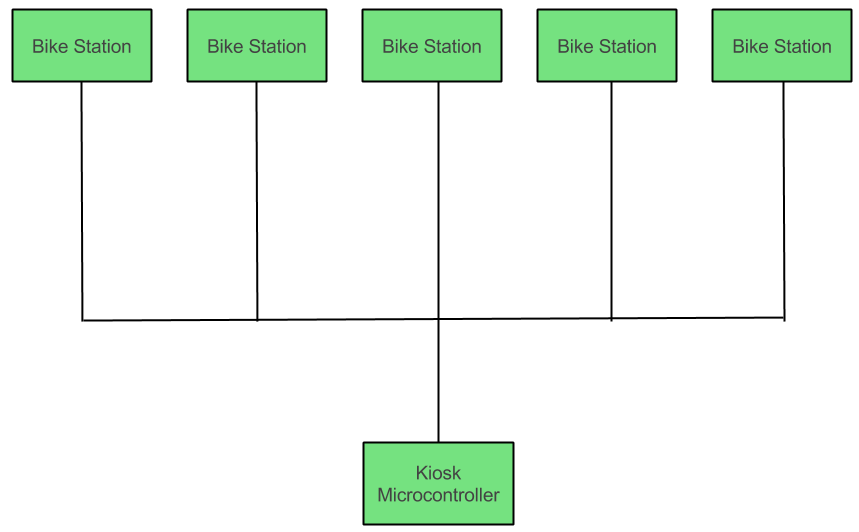
\includegraphics[scale = 0.6]{module-block-diagram}
	\end{center}
\caption{A preliminary diagram of a bike module in communication with the kiosk}

\end{figure}

In particular, Figure 2.2 displays a kiosk microcontroller communicating with 5 bike stations.  This case obviously applies to the kiosk and a single bike module.  However, as previously stated, the kiosk has the potential to communicate with up to 5 bike modules or 25 bikes.  The microcontrollers at each bike station are in direct control of their respective locking mechanisms.  In turn, each bike station controller is in direct communication with the kiosk that supplies the bike station controllers with lock, or unlock, commands.


\chapter{Component Selection}

With progress made on the communication protocol, user interactions, and locking mechanisms, components are now selected which facilitate the initial developments on each front.

\section{Communication Protocol Components}

The ABRS will communicate over a Controller Area Network (CAN) protocol.  This protocol is ubiquitous throughout automotive applications, making it an excellent choice for this type of project i.e., a central host controlling many sub-components.  Another important aspect of CAN is its communication distance.  Because there is a potential to have up to 5 modules connected to a single kiosk and assuming a module length of approximately 20 feet, the last module connected to the kiosk could be 100 feet away.  Fortunately, CAN works over distances of 500 meters at a data rate of 125 kb/s \cite{CAN protocol}.  To facilitate CAN communication, a CAN controller and CAN receiver must be purchased.  The specifics of each part are not essential.  The only important criteria is that they withstand the operating temperatures of the ABRS, which almost any embedded component can handle.  

Each component within the ABRS (e.g., kiosk, bike station) is connected to the network, as displayed in Figure 3.1.  The controller handles bus contention as well as message transmission and reception, simplifying the communications network and eliminating unnecessary coding. 

%BIB

\begin{thebibliography}{10}

\bibitem{CAN protocol}
  
  \emph{$http://en.wikipedia.org/wiki/CAN\_bus$}.
  August 1, 2014

\end{thebibliography}


\end{document}